\chapter{Principal Component Analysis}
\label{chapter:principal_component_analysis}

Combining the concepts in section~\ref{chapter:mathematical_basics} we derive the ideas and implementation of PCA.

Assume we have gathered observations of different variables as part of an experiment. If we have $n$ variables, each having been observed $m$ times, we can create a $m \times n$ matrix of this data. The goal is to get more insight and find underlying patterns in the collected data. For $n = 2$ we could try to plot the data, with the first variable as the $x$-axis and the second as the $y$ axis. An exemplary plot of some data can be seen in figure~\ref{fig:some_nice_data}.

\begin{figure}
	\centering
	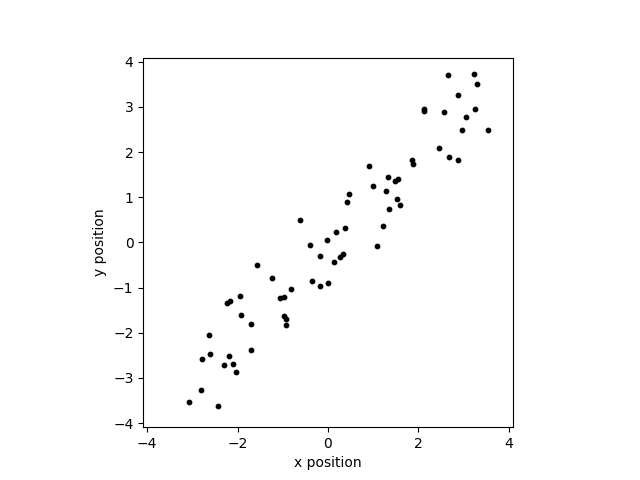
\includegraphics[width=0.8\linewidth]{figs/some_nice_data_org}
	\caption{Randomly generated sample data. The data lies along a line with slope $1$ and has mean $\mathbf{0}$.}
	\label{fig:some_nice_data}
\end{figure}

For larger values of $n$ this gets increasingly difficult\footnote{For higher dimensionality we have to use some projection. Depending on the chosen projection the interpretation changes making it difficult to interpret the resulting image.}. PCA tries to solve this problem by transforming the data in such a way that the most interesting features are in the first few axis of the transformed $m$ dimensional space. This makes it easy to look at a low dimension representation of the data, without loosing much information.

An example of PCA being applied to the data from figure~\ref{fig:some_nice_data} can be seen in figure~\ref{fig:pca_example}. In the top figure the normed data and the direction of the new axis (called Principal Components (PC)) in relation to the two original axis are shown. The bottom figure depicts the transformed data. One can see that the variance is maximal in the PC 1 axis.

\begin{figure}
	\centering
	\begin{subfigure}{0.8\linewidth}
		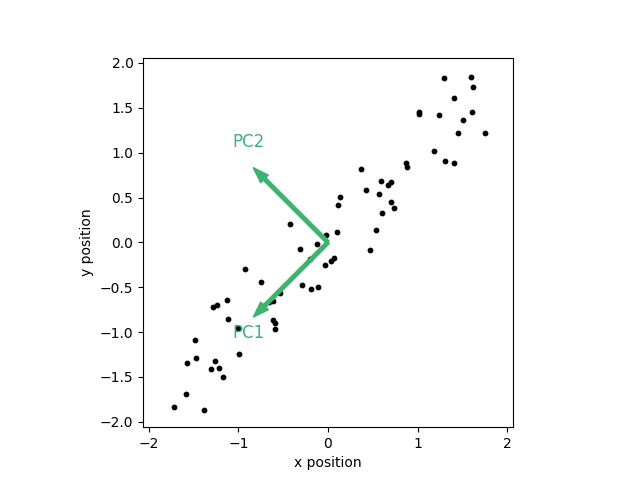
\includegraphics[width=\textwidth]{figs/some_nice_data_pc}
		\caption{Normed data (mean is zero and variance is one) and direction of the two PCs in relation to the x and y position.}
		\label{fig:some_nice_data_pc}
	\end{subfigure}
	\hfill
	\begin{subfigure}{0.8\linewidth}
		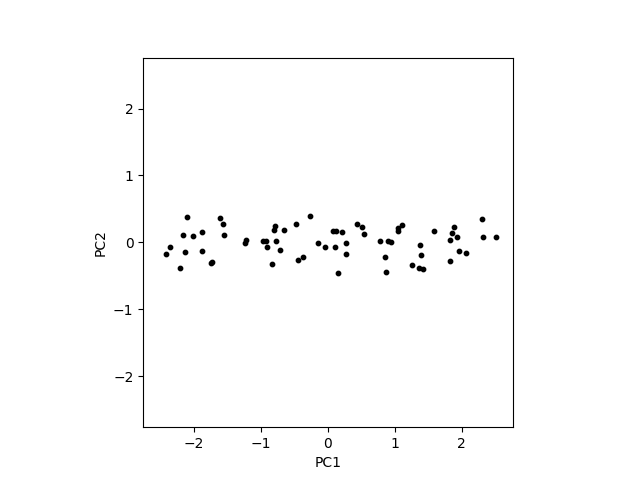
\includegraphics[width=\textwidth]{figs/some_nice_data_pca}
		\caption{The data after being transformed by PCA. The variance along the PC1 axis is maximal, therefore the data is spread out most along this axis.}
		\label{fig:some_nice_data_pca}
	\end{subfigure}
	
	\caption{Example application of PCA.}
	\label{fig:pca_example}
\end{figure}

Now we derive how to compute PCA. First we formulate a goal and define some assumptions.

We assume that the most interesting features are those that have a large variance\footnote{This assumption can be false. For data where the noise has a larger variance than the feature we are trying to observe, PCA fails because this assumption is not met.}. Our goal is to find a transformation into new coordinates such that:
\begin{itemize}
	\item the variance in the each axis is as large as possible.
	\item the axis are all orthogonal to each other.
	\item the axis are sorted (descending) by the variance in the axis.
\end{itemize}

From this we gather that another assumption is, that the axis are orthogonal. Lastly we are only concerned with linear dependent features in the data. Some example cases in which PCA fails are shown in figure~\ref{fig:pca_fails}.

\begin{figure}
	\centering
	\begin{subfigure}{0.8\linewidth}
		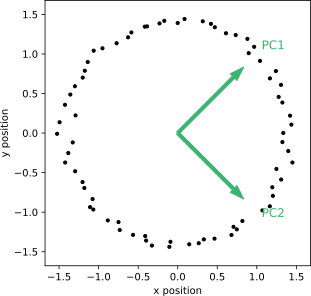
\includegraphics[width=\textwidth]{figs/pca_fails_nonlinear}
		\caption{Clearly the relationship in this figure is non-linear. PCA can not describe circular dependencies, as shown in this data.}
		\label{fig:pca_fails_nonlinear}
	\end{subfigure}
	\hfill
	\begin{subfigure}{0.8\linewidth}
		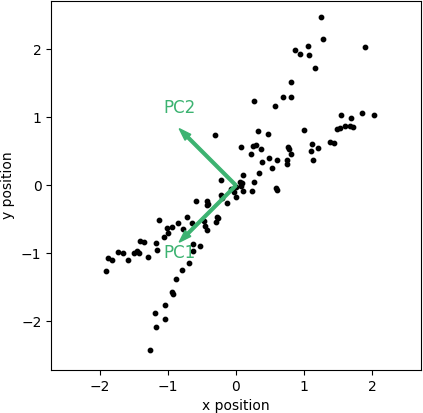
\includegraphics[width=\textwidth]{figs/pca_fails_nonorthogonal}
		\caption{The two main axis along which the data is aligned are not orthogonal to each other. PCA always outputs orthogonal principal components, therefore it fails in this example.}
		\label{fig:pca_fails_nonorthogonal}
	\end{subfigure}
	
	\caption{Examples in which some of the assumptions of PCA are not valid. The results are sub-optimal.}
	\label{fig:pca_fails}
\end{figure}

One way to achieve the goal is as follows:
\begin{enumerate}
	\item Find the direction which maximizes the variance.
	\item Save this direction as the next axis.
	\item Determine the subspace that is orthogonal to all axis we found so far.
	\item If the subspace is non-trivial start at the first step again.
	\item If the subspace is trivial we have found all axis.
\end{enumerate}

While this algorithm shows us what conceptually has to be done, we do not know how to compute the axis yet. We will now investigate this problem using the mathematical concepts from section~\ref{chapter:mathematical_basics}. This will lead us to an algorithm in which all axis can be computed simultaneously.

Let $\mathbf{X} \in \mathbbm{R}^{m\times n}$ be the data matrix. We want to find some orthonormal matrix $\mathbf{P}$ such that $\mathbf{Y}:=\mathbf{PX}$ has a diagonal covariance matrix $\mathbf{C}_{\mathbf{Y}}$.

\begin{align*}
	\mathbf{C}_{\mathbf{Y}} = \frac{1}{n}\mathbf{YY}^T = \frac{1}{n}(\mathbf{PX})(\mathbf{PX})^T = \frac{1}{n}\mathbf{PX}\mathbf{X}^T\mathbf{P}^T =\\
	= \mathbf{P}(\frac{1}{n}\mathbf{X}\mathbf{X}^T)\mathbf{P}^T = \mathbf{P}\mathbf{C}_\mathbf{X}\mathbf{P}^T
\end{align*}

The covariance matrix $\mathbf{C}_\mathbf{X}$ is symmetric and therefore has a decomposition into an orthogonal matrix of eigenvectors $\mathbf{V}$ and a diagonal matrix of eigenvalues $\mathbf{D}$. We choose $\mathbf{P}=\mathbf{V}^T$. From lemma~\ref{lem:inverse_is_transpose} it follows that $\mathbf{V}^{-1} = \mathbf{V}^T$.

\begin{align*}
	\mathbf{P}\mathbf{C}_\mathbf{X}\mathbf{P}^T = \mathbf{P}(\mathbf{VDV}^{-1})\mathbf{P}^T = \mathbf{P}(\mathbf{VDV}^{T})\mathbf{P}^T =\\
	\mathbf{P}(\mathbf{P}^T\mathbf{DP})\mathbf{P}^T = (\mathbf{P}\mathbf{P}^T)\mathbf{D}(\mathbf{P}\mathbf{P}^T) =\\
	(\mathbf{P}\mathbf{P}^{-1})\mathbf{D}(\mathbf{P}\mathbf{P}^{-1}) = \mathbf{D}
\end{align*}

In summary $\mathbf{Y}$ has a diagonal covariance matrix if we choose $\mathbf{Y} = \mathbf{V}^T\mathbf{X}$, where $\mathbf{V}$ is the matrix of eigenvectors of $\mathbf{C}_\mathbf{X}$. The eigenvectors are the PCs and the eigenvalues are the variance in each new axis.

As pseudo code we get the program from algorithm~\ref{alg:pca} for calculating the PCA.

\begin{algorithm}
	\caption{Principal Component Analysis}\label{alg:pca}
	\begin{algorithmic}
		\Require matrix $X \in \mathbbm{R}^{m\times n}$
		\State Normalize each row in the matrix $X$
		\State Calculate the covariance matrix $C_{X}$
		\State Calculate the eigenvalues and eigenvectors of $C_{X}$
		\State Sort the eigenvalues
		\State Return sorted eigenvalues and corresponding eigenvectors
	\end{algorithmic}
\end{algorithm}

What happens if we skip the step in which we normalize each row in the matrix? A big variance is interpreted by the PCA algorithm as much information, thus the variance of the variables have an impact on how ''important'' the variable is deemed. As we do not want to prioritize certain variables we avoid this behavior by normalizing the data beforehand.